% ============================================================
% 第5章：对数函数——指数的逆运算
% ============================================================

\chapter{对数函数——指数的逆运算}

\begin{applicationbox}
\textbf{学完本章你能做什么？}
\begin{enumerate}
  \item \textbf{学之前}：你学会了指数函数 \(2^x = 8\) 可以解出 \(x=3\)，但如果 \(2^x = 10\) 呢？
  \item \textbf{学之后}：你会用对数来解这类问题——"指数是多少"。你还会理解 AI 中交叉熵损失函数为什么离不开对数。
  \item \textbf{日常例子}：地震的里氏震级是对数尺度的——震级每增加 1，能量释放增加约 32 倍。
        声音的分贝也是对数尺度。对数把"天文数字"压缩成好理解的小数字。
\end{enumerate}
\end{applicationbox}


% ============================================================
\section{从第4章来——指数函数的"逆问题"}
% ============================================================

第4章我们学了指数函数 \(f(x) = a^x\)——给定底 \(a\) 和指数 \(x\)，求值 \(a^x\)。

现在问一个相反的问题：

\begin{center}
\fcolorbox{blue!40}{blue!5}{\parbox{0.8\textwidth}{
\textbf{已知底数和结果，求指数：} \\
\(2^? = 8\) —— 答案显然是 \(3\)（因为 \(2^3 = 8\)）。\\
但 \(2^? = 10\) 呢？指数是多少？
}}
\end{center}

这个问题就是\textbf{对数}要解决的。

\begin{examplebox}[1——补全对数表  🔓 完全展开]
补全下表（你能看出规律吗？）：

\begin{center}
\begin{tabular}{c|c|c|c|c|c}
\(x\) & -2 & -1 & 0 & 1 & 2 \\
\hline
\(2^x\) & 1/4 & 1/2 & 1 & 2 & 4 \\
反过来：\(? = \log_2(\text{结果})\) & \(\log_2(1/4)\) & \(\log_2(1/2)\) & \(\log_2(1)\) & \(\log_2(2)\) & \(\log_2(4)\) \\
\hline
这个"反过来的指数"等于 & -2 & -1 & 0 & 1 & 2 \\
\end{tabular}
\end{center}

\textbf{规律：} 对数 \(\log_2(y)\) 回答的是"2 的几次方等于 \(y\)"。
\textbf{为什么？} 因为对数就是指数。表格中 \(2^x\) 那一行给出的是指数运算的结果，
底下的"反过来的指数"就是底数 2 到那个结果需要的指数——也就是 \(\log_2(y)\)。
\end{examplebox}


% ============================================================
\section{对数的定义}
% ============================================================

\begin{definitionbox}[对数]
如果 \(a > 0\) 且 \(a \neq 1\)，那么
\[
a^b = c \quad\Longleftrightarrow\quad \log_a c = b
\]
读作：\textbf{以 \(a\) 为底的 \(c\) 的对数等于 \(b\)}。

其中：
\begin{itemize}
  \item \(a\) 是\textbf{底数}（base）
  \item \(c\) 是\textbf{真数}（读作 zhēn shù，必须大于 0）
  \item \(b\) 是\textbf{对数}（logarithm）
\end{itemize}
\end{definitionbox}

\begin{examplebox}[2——指数式与对数式的互化  🔒₁ 请完成最后一行]
\begin{center}
\begin{tabular}{c|c}
\textbf{指数式} & \textbf{对数式} \\
\hline
\(2^3 = 8\) & \(\log_2 8 = 3\) \\
\(3^2 = 9\) & \(\log_3 9 = 2\) \\
\(5^{-1} = 1/5\) & \(\log_5 (1/5) = -1\) \\
\(10^0 = 1\) & \(\log_{10} 1 = 0\) \\
\hline
\(a^b = c\) & \multicolumn{1}{c}{\textbf{请你写出来：}}
\end{tabular}
\end{center}

\textbf{记忆：}对数 = 指数。\(\log_a c\) 就是"把 \(a\) 变成 \(c\) 所需要的指数"。
\end{examplebox}


% ============================================================
\section{常用对数与自然对数}
% ============================================================

\begin{definitionbox}[两种最重要的对数]
\begin{enumerate}
  \item \textbf{常用对数}：底为 10，记作 \(\lg x = \log_{10} x\)。
        用于科学计算、地震震级、声音分贝。
  \item \textbf{自然对数}：底为 \(e\)，记作 \(\ln x = \log_e x\)。
        用于数学分析、AI、物理、生物学。
\end{enumerate}
\end{definitionbox}

\begin{examplebox}[3——记住几个关键值  🔒₂ 请完成最后两个]
\begin{align*}
  \lg 1 &= 0 \quad &\text{（因为 } 10^0 = 1\text{）} \\
  \lg 10 &= 1 \quad &\text{（因为 } 10^1 = 10\text{）} \\
  \lg 100 &= 2 \quad &\text{（因为 } 10^2 = 100\text{）} \\
  \\
  \ln 1 &= \quad &\text{请你写：} \\
  \ln e &= \quad &\text{请你写：}
\end{align*}
\end{examplebox}


% ============================================================
\section{对数的运算法则}
% ============================================================

\begin{theorembox}[对数运算法则]
设 \(a > 0, a \neq 1\)，\(M > 0, N > 0\)：
\begin{align*}
  \log_a (MN) &= \log_a M + \log_a N \quad &\text{（乘变加）} \\
  \log_a \frac{M}{N} &= \log_a M - \log_a N \quad &\text{（除变减）} \\
  \log_a M^n &= n \log_a M \quad &\text{（指数变系数）} \\
  \log_a \sqrt[n]{M} &= \frac{1}{n} \log_a M \quad &\text{（根号变分数）}
\end{align*}
\end{theorembox}

\begin{notebox}
\textbf{记忆口诀：}\\
乘变加，除变减，指数变系数，根号变分数。
\end{notebox}

\begin{examplebox}[4——对数运算  🔒₃ 只给开头，你来完成]
计算：
\[
(1)\; \lg 2 + \lg 5 \qquad (2)\; \log_2 8 - \log_2 2 \qquad (3)\; \log_3 9^2
\]

\textbf{给你一个开头：}
\[
(1)\; \lg 2 + \lg 5 = \lg(2 \times 5) = \lg 10 = 1
\]

\textbf{你来完成 (2) 和 (3)：} 使用对数运算法则（乘变加、除变减、指数变系数）。
写出每一步的依据。完成后用下面方法验算：
\[
\log_3 81 = ? \quad (\text{因为 } 3^? = 81)
\]
\end{examplebox}

% ── 信心校准（渐退序列中段）──
\begin{confidencebox}
从例1（完全展开）到例4（只给开头），你感觉到难度递增了吗？
如果例4卡住了，说明对数运算法则还不够熟——回看本节定理框，把"乘变加、除变减、指数变系数"默写一遍。
\end{confidencebox}


\begin{examplebox}[5——换底公式]
\textbf{换底公式}（重要）：
\[
\log_a b = \frac{\log_c b}{\log_c a}
\]

特别地：\(\log_a b = \frac{\ln b}{\ln a} = \frac{\lg b}{\lg a}\)

\textbf{例：} 计算 \(\log_2 5\)（用计算器算 \(\ln 5\) 和 \(\ln 2\)）：
\[
\log_2 5 = \frac{\ln 5}{\ln 2} \approx \frac{1.6094}{0.6931} \approx 2.3219
\]

验证：\(2^{2.3219} \approx 5\) [OK]
\end{examplebox}


% ============================================================
\section{对数函数 \(y = \log_a x\)}
% ============================================================

\begin{definitionbox}[对数函数]
形如
\[
f(x) = \log_a x \quad (a > 0,\; a \neq 1,\; x > 0)
\]
的函数称为\textbf{对数函数}（读作 duì shù hán shù，英文 logarithmic function）。

它是\textbf{指数函数 \(a^x\) 的反函数}。
\end{definitionbox}

\subsection{底 > 1：增长型对数函数}

\begin{examplebox}[6]
对比 \(y = \log_2 x\)、\(y = \ln x\)、\(y = \lg x\)：

\begin{center}
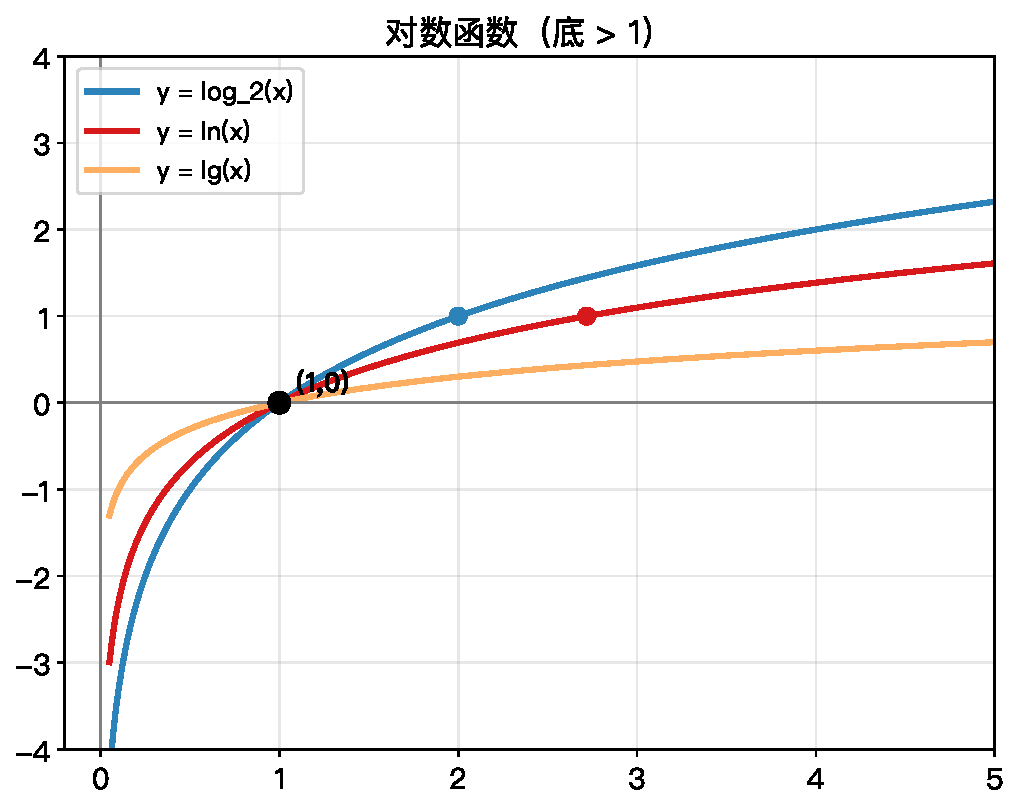
\includegraphics[width=0.6\textwidth]{figures/ch05_logarithm_bases.pdf}
\end{center}

\textbf{观察规律：}
\begin{enumerate}
  \item 所有对数函数都经过 \((1,0)\)——因为 \(\log_a 1 = 0\)
  \item 所有对数函数都经过 \((a,1)\)——因为 \(\log_a a = 1\)
  \item 底越大，增长越\textbf{慢}（\(\log_2 x\) 比 \(\lg x\) 增长快）
  \item 定义域：\(x > 0\)（负数没有对数）
  \item 值域：\(\mathbb{R}\)（全体实数）
  \item 垂直渐近线：\(x = 0\)（当 \(x \to 0^+\) 时，\(\log_a x \to -\infty\)）
\end{enumerate}
\end{examplebox}

\subsection{0 < 底 < 1：衰减型对数函数}

\begin{examplebox}[7]
\begin{center}
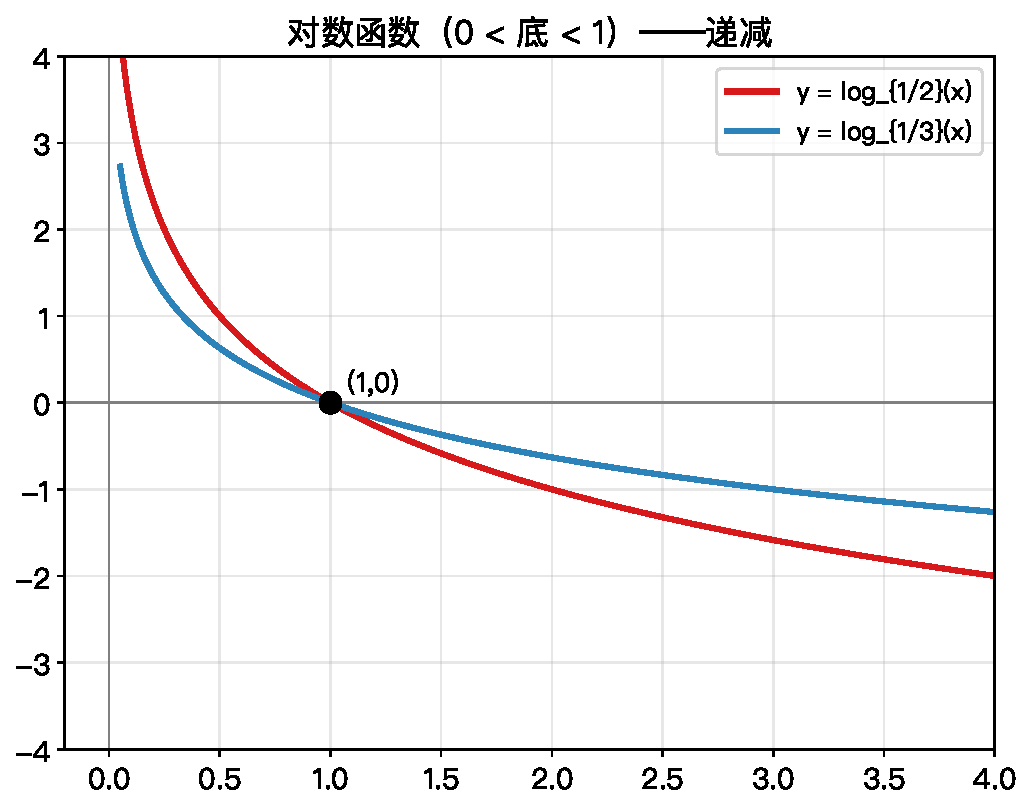
\includegraphics[width=0.6\textwidth]{figures/ch05_logarithm_decay.pdf}
\end{center}

\textbf{对比底>1：}
\begin{itemize}
  \item 还是经过 \((1,0)\)——但现在是\textbf{递减}的
  \item 底越小，衰减越快
  \item 当 \(x \to 0^+\) 时，\(\log_a x \to +\infty\)（与底>1相反）
\end{itemize}
\end{examplebox}


% ============================================================
\section{指数与对数——互逆关系}
% ============================================================

指数函数和对数函数是\textbf{互为反函数}的关系。

\begin{theorembox}[指数与对数的互逆]
如果 \(f(x) = a^x\)，那么它的反函数是 \(f^{-1}(x) = \log_a x\)。

两者的图像关于直线 \(y = x\) 对称：
\[
(a^x \text{ 上的点 } (b, a^b)) \;\longleftrightarrow\; (\log_a x \text{ 上的点 } (a^b, b))
\]
\end{theorembox}

\begin{examplebox}[8]
\(y = 2^x\) 和 \(y = \log_2 x\) 关于 \(y = x\) 对称：

\begin{center}
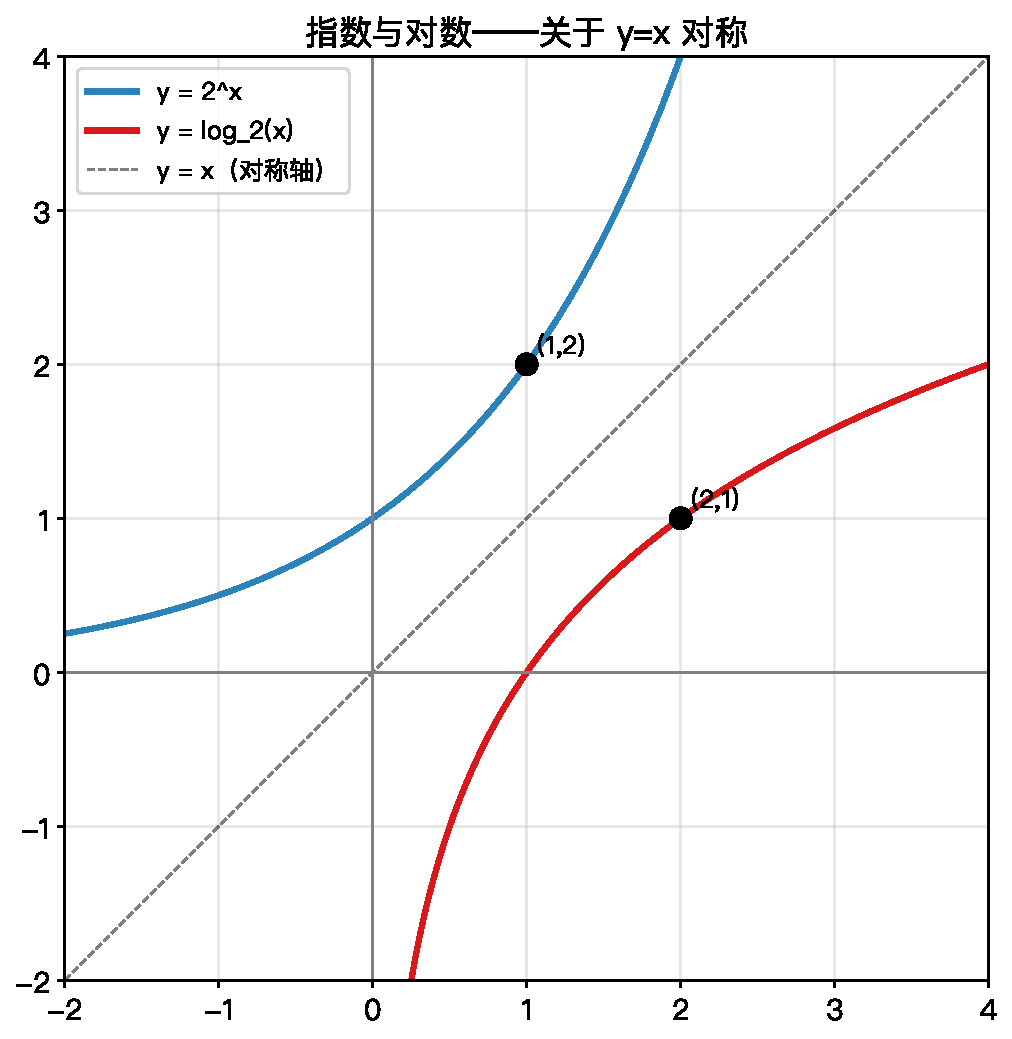
\includegraphics[width=0.55\textwidth]{figures/ch05_exp_log_inverse.pdf}
\end{center}

\textbf{具体验证：}
\[
2^3 = 8 \;\Longrightarrow\; (3, 8) \text{ 在 } y=2^x \text{ 上}
\]
\[
\log_2 8 = 3 \;\Longrightarrow\; (8, 3) \text{ 在 } y=\log_2 x \text{ 上}
\]

两个点的坐标互换了位置——这就是\textbf{反函数}的本质。
\end{examplebox}


% ============================================================
\section{对数的"压缩"效果}
% ============================================================

对数有一个重要的实际作用——\textbf{把大数压缩成小数}。

\begin{examplebox}[9]
\begin{center}
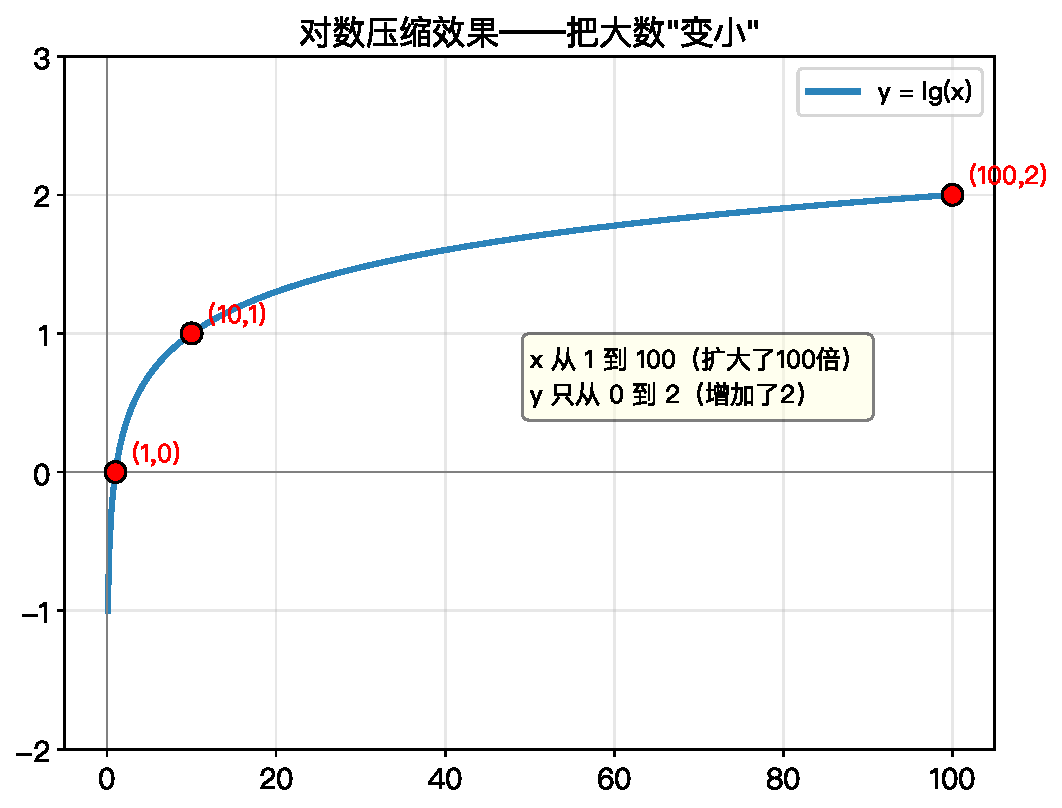
\includegraphics[width=0.55\textwidth]{figures/ch05_log_compression.pdf}
\end{center}

\textbf{看这个表：}
\begin{center}
\begin{tabular}{c|c}
\(x\) & \(\lg x\) \\
\hline
1 & 0 \\
10 & 1 \\
100 & 2 \\
1000 & 3 \\
1,000,000 & 6 \\
1,000,000,000 & 9 \\
\end{tabular}
\end{center}

\(x\) 从 1 扩大到 10 亿（扩大了 10 亿倍），\(\lg x\) 只从 0 增加到 9（增加了 9）。\\
这就是\textbf{对数压缩}——把天文数字变成好处理的小数字。

\textbf{应用：}地震震级（里氏 6 级比 5 级能量大约 32 倍）、声音分贝、pH 值、AI 中的交叉熵。
\end{examplebox}


% ============================================================
\section{对数方程与不等式}
% ============================================================

\begin{definitionbox}[对数方程]
真数中含有未知数的方程叫\textbf{对数方程}。

解法：利用对数的定义和运算法则，转化为普通方程。

\textbf{注意：}解出来之后一定要\textbf{验根}——真数必须大于 0！
\end{definitionbox}

\begin{examplebox}[10——解对数方程]
解方程：
\[
(1)\; \log_2 x = 3 \qquad (2)\; \lg(x+1) + \lg(x-1) = \lg 3
\]

解：
\[
\begin{aligned}
(1)&\; \log_2 x = 3 \;\Longrightarrow\; x = 2^3 = 8 \\
   &\;\text{验根：} x = 8 > 0 \;\text{[OK]}
\end{aligned}
\]

\[
\begin{aligned}
(2)&\; \lg(x+1) + \lg(x-1) = \lg 3 \\
   &\;\lg[(x+1)(x-1)] = \lg 3 \\
   &\;(x+1)(x-1) = 3 \\
   &\;x^2 - 1 = 3 \;\Longrightarrow\; x^2 = 4 \;\Longrightarrow\; x = \pm 2 \\
   &\;\text{验根：} x = 2 \text{ 时，} x+1 > 0,\; x-1 > 0 \;\text{[OK]} \\
   &\;\text{验根：} x = -2 \text{ 时，} x-1 = -3 < 0 \;\text{（真数不能为负）[X]} \\
   &\;\text{所以 } x = 2 \text{ 是唯一解。}
\end{aligned}
\]
\end{examplebox}


% ============================================================
\section{对数在 AI 中的应用——交叉熵损失}
% ============================================================

\begin{examplebox}[11——交叉熵损失函数]
在 AI 分类任务中，模型输出一个概率分布，我们需要衡量"预测分布"和"真实分布"的差距。

\[
\text{Loss} = -\sum_{i} y_i \log(p_i)
\]

其中 \(y_i\) 是真实标签（0 或 1），\(p_i\) 是模型预测的概率。

\textbf{为什么用对数？}
\begin{enumerate}
  \item 当 \(p_i\) 接近 1（预测正确）时，\(\log(p_i) \approx 0\)，loss 很小
  \item 当 \(p_i\) 接近 0（预测错误）时，\(\log(p_i) \to -\infty\)，loss 很大
  \item 对数放大了"错误预测"的惩罚——模型会拼命避免犯错
\end{enumerate}

\textbf{例：} 真实标签 \(y = [1, 0, 0]\)，预测 \(p = [0.8, 0.15, 0.05]\)：
\[
\text{Loss} = -(1\cdot\ln 0.8 + 0\cdot\ln 0.15 + 0\cdot\ln 0.05) = -\ln 0.8 \approx 0.223
\]
\end{examplebox}


% ============================================================
\section{符号卡片}
% ============================================================

\begin{symbolcard}
\(\log_a c\) & \verb|\log_a c| & 读作"以 a 为底 c 的对数" & \(a\) 的几次方等于 \(c\) \\
\(\lg x\) & \verb|\lg x| & 读作"常用对数 x" & \(\log_{10} x\)，底为 10 \\
\(\ln x\) & \verb|\ln x| & 读作"自然对数 x" & \(\log_e x\)，底为 \(e\) \\
真数 & —— & 读作"zhēn shù" & 对数中的 \(c\)，必须 \(> 0\) \\
\end{symbolcard}


% ============================================================
\section{代码验证}
% ============================================================

\begin{lstlisting}[caption=对数函数的数值验证]
import numpy as np

# 1. 验证指数和对数的互逆关系
print("=== 指数与对数互逆 ===")
for x in [1, 2, 3, 4, 5]:
    exp_val = 2**x
    log_val = np.log2(exp_val)
    print(f"  2^{x} = {exp_val:3d},  log2({exp_val:3d}) = {log_val}")

print()

# 2. 验证对数运算法则
print("=== 对数运算法则 ===")
print(f"  lg(2) + lg(5) = {np.log10(2) + np.log10(5):.4f}")
print(f"  lg(10)       = {np.log10(10):.4f}")
print(f"  log2(8*4)    = {np.log2(8*4):.4f}  (应等于 log2(8)+log2(4) = {np.log2(8)+np.log2(4):.4f})")

print()

# 3. 交叉熵损失模拟
def cross_entropy(y_true, y_pred):
    """计算交叉熵损失"""
    # 防止 log(0)
    eps = 1e-15
    y_pred = np.clip(y_pred, eps, 1 - eps)
    return -np.sum(y_true * np.log(y_pred))

print("=== 交叉熵损失 ===")
y_true = np.array([1, 0, 0])
good_pred = np.array([0.95, 0.03, 0.02])
bad_pred = np.array([0.3, 0.4, 0.3])
print(f"  正确预测的损失: {cross_entropy(y_true, good_pred):.4f}")
print(f"  错误预测的损失: {cross_entropy(y_true, bad_pred):.4f}")
print(f"  完美预测的损失: {cross_entropy(y_true, np.array([1, 0, 0])):.4f}")
\end{lstlisting}

运行结果：
\begin{lstlisting}[frame=none,backgroundcolor={},numbers=none]
=== 指数与对数互逆 ===
  2^1 =   2,  log2(  2) = 1.0
  2^2 =   4,  log2(  4) = 2.0
  2^3 =   8,  log2(  8) = 3.0
  2^4 =  16,  log2( 16) = 4.0
  2^5 =  32,  log2( 32) = 5.0

=== 对数运算法则 ===
  lg(2) + lg(5) = 1.0000
  lg(10)       = 1.0000
  log2(8*4)    = 5.0000  (应等于 log2(8)+log2(4) = 5.0000)

=== 交叉熵损失 ===
  正确预测的损失: 0.0513
  错误预测的损失: 1.2040
  完美预测的损失: 0.0000
\end{lstlisting}


% ============================================================
\section{本章小结}
% ============================================================

\begin{progressbox}
\textbf{对数的定义}：\(a^b = c \;\Longleftrightarrow\; \log_a c = b\)——对数就是指数。

\textbf{运算法则}：乘变加、除变减、指数变系数

\textbf{对数函数} \(y = \log_a x\)：
\begin{itemize}
  \item 定义域 \(x > 0\)，值域 \(\mathbb{R}\)，经过 \((1,0)\) 和 \((a,1)\)
  \item 底 > 1：递增；0 < 底 < 1：递减
  \item 垂直渐近线 \(x = 0\)
\end{itemize}

\textbf{指数与对数互逆}：\(y = a^x\) 和 \(y = \log_a x\) 关于 \(y = x\) 对称

\textbf{对数压缩}：把天文数字变成小数字——地震震级、分贝、交叉熵

\textbf{AI 应用}：交叉熵损失函数用对数放大错误惩罚
\end{progressbox}

\subsection*{通往下一章}

\textbf{这一章}你学会了对数函数——指数的逆运算。

\textbf{下一章}我们将进入\textbf{三角函数}——描述周期运动的数学工具。
从声音的波形到地球绕太阳公转，再到 AI 中的位置编码（Transformer），
三角函数无处不在。


% ============================================================
% 习题
% ============================================================
\section{习题}

% ===== 送分 =====

\begin{exercise}[0]
将指数式化为对数式：
\[
(1)\; 2^4 = 16 \qquad (2)\; 3^3 = 27 \qquad (3)\; 10^2 = 100
\]
\end{exercise}

\begin{exercise}[0]
将对数式化为指数式：
\[
(1)\; \log_2 8 = 3 \qquad (2)\; \log_3 81 = 4 \qquad (3)\; \lg 1000 = 3
\]
\end{exercise}

\begin{exercise}[0]
求值：
\[
(1)\; \lg 10 \qquad (2)\; \ln e \qquad (3)\; \log_5 25 \qquad (4)\; \log_2 1
\]
\end{exercise}
\qquad \textcolor{gray}{[回顾第4章：指数与对数的互逆]}%

\begin{exercise}[0]
判断正误：
\[
(1)\; \lg 100 = 2 \qquad (2)\; \ln 1 = 1 \qquad (3)\; \log_3 9 = 2 \qquad (4)\; \log_2 0 = 0
\]

% ===== 简单 =====

\end{exercise}

\begin{exercise}[1]
用 \(\lg 2\) 和 \(\lg 3\) 表示：
\[
(1)\; \lg 6 \qquad (2)\; \lg \frac{2}{3} \qquad (3)\; \lg 8
\]
\end{exercise}

\begin{exercise}[1]
计算：
\[
(1)\; \lg 20 - \lg 2 \qquad (2)\; \log_3 5 + \log_3 \frac{1}{5} \qquad (3)\; \ln e^3
\]
\end{exercise}

\begin{exercise}[1]
画出 \(y = \log_2 x\) 的草图（取 \(x = 1/2, 1, 2, 4\) 四个点）。
标出它与 \(x\) 轴的交点。

\end{exercise}
\qquad \textcolor{gray}{[回顾第2章：图像法]}%

\begin{exercise}[1]
填空：对数函数 \(y = \log_a x\)（\(a > 1\)）的定义域是\_\_\_\_，值域是\_\_\_\_，\\
当 \(x > 1\) 时 \(y\)\_\_\_\_0，当 \(0 < x < 1\) 时 \(y\)\_\_\_\_0。

% ===== 基础 =====

\end{exercise}

\begin{exercise}[2]
计算：
\[
(1)\; \log_2 16 + \log_2 \frac{1}{8} \qquad (2)\; \lg 25 + \lg 4 \qquad (3)\; \log_3 54 - \log_3 2
\]
\end{exercise}

\begin{exercise}[2]
解方程：
\[
(1)\; \log_3 x = 2 \qquad (2)\; \lg(x-1) = 0 \qquad (3)\; \ln(2x) = 1
\]
\end{exercise}

\begin{exercise}[2]
用换底公式计算（保留两位小数）：
\[
(1)\; \log_2 10 \qquad (2)\; \log_5 3
\]
（提示：\(\log_a b = \frac{\lg b}{\lg a}\)）

\end{exercise}

\begin{exercise}[2]
比较大小：
\[
(1)\; \log_2 3 \text{ 和 } \log_2 5 \qquad
(2)\; \log_{0.5} 3 \text{ 和 } \log_{0.5} 5
\]

% ===== 普通 =====

\end{exercise}
\qquad \textcolor{gray}{[回顾第4章：指数函数单调性]}%

\begin{exercise}[3]
已知 \(\lg 2 \approx 0.3010\)，\(\lg 3 \approx 0.4771\)，求：
\[
(1)\; \lg 6 \qquad (2)\; \lg 12 \qquad (3)\; \lg 1.5
\]
\end{exercise}
\begin{hintref}本题 L2：用哪个定理——参见本章提示附录。\end{hintref}

\begin{exercise}[3]
解方程：
\[
\lg(x+2) + \lg(x-2) = \lg 5
\]
（注意验根！）

\end{exercise}
\begin{hintref}本题 L2：用哪个定理——参见本章提示附录。\end{hintref}

\begin{exercise}[3]
地震的里氏震级 \(M\) 和能量 \(E\)（焦耳）的关系为 \(\lg E = 4.8 + 1.5M\)。
\begin{enumerate}
  \item[(1)] 震级 5 级的地震释放多少能量？
  \item[(2)] 震级 6 级比 5 级能量大多少倍？
\end{enumerate}

\end{exercise}
\begin{hintref}本题 L2：用哪个定理——参见本章提示附录。\end{hintref}
\qquad \textcolor{gray}{[回顾第1章：函数建模]}%

\begin{exercise}[3]
化简：
\[
\log_2 3 \times \log_3 4 \times \log_4 5
\]
（提示：用换底公式写成 \(\frac{\lg 3}{\lg 2} \times \frac{\lg 4}{\lg 3} \times \cdots\)）

\end{exercise}
\begin{hintref}本题 L2：用哪个定理——参见本章提示附录。\end{hintref}

\begin{exercise}[3]
证明 \(\log_a b = \dfrac{1}{\log_b a}\)（\(a,b > 0, a\neq1, b\neq1\)）。

% ===== 中等 =====

\end{exercise}
\begin{hintref}本题 L2：用哪个定理——参见本章提示附录。\end{hintref}

\begin{exercise}[4]
解方程：
\[
(1)\; \log_2(x+1) + \log_2(x-1) = 3 \qquad
(2)\; \lg^2 x - \lg x - 2 = 0
\]
（提示：(2) 令 \(t = \lg x\)）

\end{exercise}
\begin{hintref}本题 L3+L4：第一步+完整思路——参见本章提示附录。\end{hintref}

\begin{exercise}[4]
已知函数 \(f(x) = \ln(x + \sqrt{1 + x^2})\)。
\begin{enumerate}
  \item[(1)] 求 \(f(0)\)、\(f(1)\)、\(f(-1)\)
  \item[(2)] 判断 \(f(x)\) 是奇函数还是偶函数
\end{enumerate}

\end{exercise}
\begin{hintref}本题 L3+L4：第一步+完整思路——参见本章提示附录。\end{hintref}

\begin{exercise}[4]
已知 \(\log_2 3 = a\)，\(\log_3 5 = b\)，用 \(a, b\) 表示 \(\log_2 15\)。

\end{exercise}
\begin{hintref}本题 L3+L4：第一步+完整思路——参见本章提示附录。\end{hintref}

\begin{exercise}[4]
函数 \(y = \log_2(x-1) + 2\) 是由 \(y = \log_2 x\) 经过怎样的平移得到的？
它的定义域和值域分别是什么？

\end{exercise}
\begin{hintref}本题 L3+L4：第一步+完整思路——参见本章提示附录。\end{hintref}

\begin{exercise}[4]
解不等式：
\[
(1)\; \log_2 x > 3 \qquad (2)\; \log_{0.5} x \ge -2
\]

% ===== 进阶 =====

\end{exercise}
\begin{hintref}本题 L3+L4：第一步+完整思路——参见本章提示附录。\end{hintref}

\begin{exercise}[5]
解方程 \(\log_2(4^x + 4) = x + \log_2(2^{x+1} - 3)\)。
（提示：利用对数运算法则拆开，再换元）

\end{exercise}
\begin{hintref}本题 L3+L4：第一步+完整思路——参见本章提示附录。\end{hintref}

\begin{exercise}[5]
已知函数 \(f(x) = \ln \dfrac{1-x}{1+x}\)（\(-1 < x < 1\)）。
\begin{enumerate}
  \item[(1)] 判断 \(f(x)\) 的奇偶性
  \item[(2)] 证明 \(f(a) + f(b) = f\left(\dfrac{a+b}{1+ab}\right)\)
\end{enumerate}

\end{exercise}
\begin{hintref}本题 L3+L4：第一步+完整思路——参见本章提示附录。\end{hintref}

\begin{exercise}[5]
某声音的强度是 \(I\) 瓦/平方米，其分贝值为 \(d = 10 \lg \dfrac{I}{I_0}\)，
其中 \(I_0 = 10^{-12}\)（人耳能听到的最小声）。
\begin{enumerate}
  \item[(1)] 正常谈话的强度 \(I = 10^{-6}\)，求分贝值
  \item[(2)] 摇滚音乐会 \(I = 1\)，求分贝值
  \item[(3)] 分贝每增加 10，强度扩大多少倍？
\end{enumerate}

\end{exercise}
\begin{hintref}本题 L3+L4：第一步+完整思路——参见本章提示附录。\end{hintref}
\qquad \textcolor{gray}{[回顾第4章：对数与指数的互逆]}%

\begin{exercise}[5]
已知 \(a > 0, a \neq 1\)，比较 \(\log_a (a^2 + 1)\) 和 \(\log_a (2a)\) 的大小。

% ===== 拔高 =====

\end{exercise}
\begin{hintref}本题 L3+L4：第一步+完整思路——参见本章提示附录。\end{hintref}

\begin{exercise}[6]
已知函数 \(f(x) = \log_2 (x^2 - 2ax + 3)\)。
\begin{enumerate}
  \item[(1)] 若 \(f(x)\) 的定义域为 \(\mathbb{R}\)，求 \(a\) 的取值范围
  \item[(2)] 若 \(f(x)\) 的值域为 \(\mathbb{R}\)，求 \(a\) 的取值范围
\end{enumerate}

\end{exercise}
\begin{hintref}本题 L2+L3+L4：知识点梳理+第一步+完整思路——参见本章提示附录。\end{hintref}

\begin{exercise}[6]
解方程 \(\log_2 (x+1) = \log_4 (x+5)\)。
（提示：把两边的底数统一，用换底公式）

\end{exercise}
\begin{hintref}本题 L2+L3+L4：知识点梳理+第一步+完整思路——参见本章提示附录。\end{hintref}

\begin{exercise}[6]
已知 \(\log_{12} 27 = a\)，用 \(a\) 表示 \(\log_6 16\)。
（提示：先把 \(\log_{12} 27\) 写成常用对数形式，再解出 \(\lg 3 / \lg 2\) 的关系）

% ===== 极难 =====

\end{exercise}
\begin{hintref}本题 L2+L3+L4：知识点梳理+第一步+完整思路——参见本章提示附录。\end{hintref}

\begin{exercise}[7]
已知函数 \(f(x) = \lg \dfrac{1 - x}{1 + x}\)。
\begin{enumerate}
  \item[(1)] 求 \(f(x)\) 的定义域
  \item[(2)] 判断奇偶性并证明
  \item[(3)] 解不等式 \(f(x) > 0\)
  \item[(4)] 已知 \(f(a) + f(b) = f(c)\)，用 \(a, b\) 表示 \(c\)
\end{enumerate}

\textbf{说明：} 这道题把定义域、奇偶性、不等式、对数运算综合在一起，
每一步都需要用到本章的不同知识点。
\end{exercise}

% ── 先想后看门禁 ──
\begin{retrievalgatebox}
翻答案之前，先做三件事：
\begin{enumerate}
  \item 用一句话说出本章核心概念。
  \item 有做错的题？找一道同类型、同难度的新题（从本章习题中选一道没做过的），独立做一遍。
  \item 选一道做对的题，讲给想象中的初学者听。
\end{enumerate}
\end{retrievalgatebox}

% ── 信心校准（习题区末尾）──
\begin{confidencebox}
做完本章后，你能用自己的话解释「对数是指数的逆运算」吗？
如果能，你确实学会了。如果不行，重读例1、例2和例8。
\end{confidencebox}

\begin{hintref}本题 L2+L3+L4：知识点梳理+第一步+完整思路——参见本章提示附录。\end{hintref}
